\documentclass[a4paper]{report}
\usepackage{master}
\begin{document}

\author{Тузова Екатерина}
\title{Ebooks searching, reading, managing system}

\maketitle
%TODO сделать тире
% подумать про заголовки


\abstract{
Мотивацией для данного проекта послужило желание облегчить работу пользователей с электронными книгами. Ресурсы, которые сейчас есть в интеренете, позволяют пользователю последовательно сначала находить нужную книгу, затем самостоятельно скачивать и искать программу, которая может работать с файлом в заданном формате.

Основная идея проекта - избавить пользователя от лишних и трудоемких действий, оставив ему самую приятную часть - непосредственно чтение книги. Таким образом, проект призван объединить все стадии подготовки к чтению(поиск, скачивание, открытие файла) в одну. }

\newpage
\tableofcontents
\newpage

\numlesschap{Введение}
В последние годы влияние Интернета на жизнь человека становится все сильнее. Это обусловлено тем, что Интернет предоставляет гораздо больше удобства и возможностей для доступа к информации. Не оказалась в стороне от Интернета и такая важная часть работы и досуга, как чтение книг.

 Если 20 лет назад человек хотел почитать книгу, он шел в библиотеку или в книжный магазин. Если он искал определённую книгу - достаточно было назвать фамилию автора и название книги, а порой одного названия было достаточно. Если же выбор книги ещё не был сделан, всегда можно было получить помощь от сотрудника магазина или библиотеки. Сегодня ситуация с библиотеками и книжными магазинами изменилась несильно. 

Наравне с бумажными книгами появилась возможность читать книги в электронном виде. Большое количество книг оцифровано и хранится в сети Интернет, многие из них в свободном доступе. С одной стороны это должно упрощать процесс получения книг, теперь они стали доступны из любого места, где есть возможность выхода в Интернет. С другой стороны, перед пользователем встает новая проблема - теперь ему необходимо самому искать эту книгу в сети, где количество информации растет с каждым днем. Но эта проблема не единственна. После того, как он нашел нужную книгу - ее нужно скачать, а затем найти программу, которая может работать с файлом в найденном формате. 

%TODO 
На настоящий момент в Интернете существует множество электронных библиотек, поиск по которым весьма затруднен из-за того, что не существует системы, которая могла бы объединить всю информацию с этих библиотек. Поэтому пользователям приходится либо искать в каждой из электронных библиотек в отдельности, либо пользоваться существующими поисковыми системами. Вторая проблема, связанная с наличием большого количества электронных библиотек в том, что единый формат для предоставления информации о книгах появился только недавно. 

У существующих поисковых систем есть одна очень важная особенность - они обладают ограниченными возможностями в проведении специализированного поиска в сети. Поэтому при поиске пользователь получает всю информацию, которая соответствует поисковому запросу. И дальше уже начинается работа самого пользователя над тем, чтобы эту информацию профильтровать и извлечь оттуда именно то, что ему нужно. 

Таким образом, выявляются две важные проблемы, затрудняющие поиск книг. Первая проблема - различные библиотеки имеют разные интерфейсы, вторая - существует множество форматов, в которых может быть представлена электронная книга. 

В данной работе была разработана система, упрощающая задачу поиска, чтения и управления книгами. 


\numlesschap{Обзор существующих решений}

Уже предпринимались попытки решить эти проблемы.

Например, широко известная поисковая система Google предоставляет свой сервис для поиска электронных книг - Google books (\url{http://books.google.com}). Этот сервис выполняет полнотекстовый поиск по книгам, которые Google сканирует и сохраняет в своей базе данных. В качестве результатов выдается большое количество информации о самой книге, об изданиях этой книги и ссылки на ресурсы, где пользователь может купить эту книгу. Благодаря полнотекстовому поиску  по содержанию, есть возможность найти книгу, имея сильно ограниченное количество информации о ней. Это не решает ни проблему унифицированного доступа к информации о книгах, ни проблему различных форматов книг.

Например, ebdb.ru(electronics books data base)  - это поисковая система, которая обходит интернет и сохраняет у себя ссылки на страницы других ресурсов, содержащие ссылки на книги. В результате поиска выдается список ссылок на страницы, содержащие книги. Для того, чтобы получить книгу пользователь должен перейти по ссылке, и, возможно, зарегистрироваться на ресурсе. Это решает проблему поиска книг, находящихся в свободном доступе, но остаются другие задачи, которые пользователь вынужден выполнять сам (скачивание книг, и поиск подходящей программы для просмотра). Так же эта поисковая система не решает проблемы унифицированного доступа и проблему различных форматов книг.

Есть большие системы, решающие проблему унифицированного доступа и различных форматов книг, а именно, Amazon Kindle, Sony Reader и подобные. 
Это программно-аппаратные платформы для чтения электронных книг. Они предоставляют устройство, которое имеет доступ к определенному хранилищу. Пользователь может подключить свое устройство к Интернету, найти нужную книгу в этом хранилище и купить ее. Дальше устройство само скачает эту книгу и откроет ее.
Из минусов у таких систем то, что это платные системы и зависимые от устройства. Так же количество доступных книг - ограничено теми книгами, которые хранят/продают хранилища, к которым они подключаются. Но это не единственные минусы таких систем, так у Amazon Kindle за каждый загруженный текст (вне зависимости от источника загрузки) требуется заплатить компании Amazon от 10 центов. Еще Amazon контролирует информацию, содержащуюся на устройствах, находящихся у пользователей и по своему усмотрению удаляет её (в том числе книги, приобретённые непосредственно у Amazon).

Существует открытая технология, решающая проблему унифицированного доступа  - OPDS (Open Publication Distribution System).
OPDS - это новый активно развивающийся стандарт, который построен на базе расширяемого языка разметки Atom. Этот стандарт был специально разработан для предоставления информации об электронных документах. В стандарте учтены особенности такого рода информации (наличие аннотации, автора, изображения обложки и пр.).
Основная идея существования такого стандарта в том, что если многие сайты будут распостранять свою информацию о книгах в таком формате, то клиентские программы могут подключаться к большому количеству сайтов. Несмотря на то, что стандарт появился недавно, уже существуют сайты и клиетские программы, использующие этот протокол. 

\begin{figure}
\centering
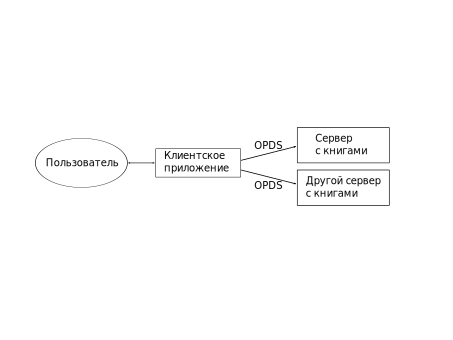
\includegraphics[width=.5\textwidth]{scheme}
\caption{Схема взаимодействия с использованием формата OPDS}\label{fig:scheme}
\end{figure}

Одим из самых крупных сайтов, предоставляющих информацию по протоколу OPDS, является BookServer (\url{http://bookserver.archive.org}).
Этот некоммерческий проект является частью проекта Internet Archive (\url{http://archive.org}) и является универсальной и открытой системой распостранения электронных книг. BookServer это архитектура, объединяющая различные форматы книг, конвертируя их, при необходимости, в нужный формат. Система обеспечивает каталогизацию книг, имеющихся в магазинах, библиотеках или в открытом доступе. Электронный текст можно прочитать на любом конечном устройстве, будь то нетбук, смартфон или специализированное устройство для чтения, наподобие Kindle. Хотя сайтом уже можно пользоваться, он еще находится на стадии разработки, с чем, вероятно, связано отсутствие расширенного поиска по книгам, фильтрации по языкам/жанрам. 

%STOP
\numlesschap{Описание системы в целом}
Проект состоит из серверной и клиентской частей.

Серверная часть собирает в сети Интернет информацию об электронных книгах и представляет собранную информацию для обычных пользователей в виде web-интерфейса и для клиентских программ -- в формате OPDS.

Клиентская часть представляет собой программу для удобной работы с сервером, предоставляющим по запросам информацию в формате OPDS. Клиент должен работать как с "родным" сервером, так и с другими серверами, поддерживающими OPDS, например feedbooks.com.

Серверная часть проекта состоит из 3 подпроектов:
\begin{itemize}
\item собственно web-сервер, включающий базу данных, поиск по ней, представление информации в web и opds форматах (python, django)
\item сборщик информации в сети (crawler) (java)
\item анализатор найденной информации, разбирающий информацию о книгах (java) 
\end{itemize}
Клиентских программ написано 2:
\begin{itemize}
\item На С++ (с интерфейсом Qt)
\item На Java 
\end{itemize}

Клиентская программа на Java более переносима, но для нее необходимо на девайсе иметь java-машину. В свою очередь программа на Qt не требует установки никаких дополнительных библиотек, работает быстрее, но переносимость ниже, чем у java.
		
\numlesschap{Описание компонентов системы и их взаимодействие}

% Может стоит вставить пару картинок

Пользователь устанавливает у себя на машине одну из клиентских программ. При поиске книги программа обращается к одному из серверов, поддерживающих протокол OPDS,(OpenSearch?). Сервер обрабатывает запрос, и возвращает данные в в нужном формате. Счастливый пользователь может читать книгу.


\numlesschap{Постановка задачи}

После того, как книги найдены и добавлены в базу данных появляются новые задачи - это предоставление информации конечному пользователю, а так же верификация и обновление данных. С предоставлением информации пользователю все более-менее ясно. Базу данных нужно все время поддерживать в рабочем состоянии. А информация, поступающая от crawler'a с analyzer'ом зачастую бывает весьма сомнительного качества. Иногда, crawler находит книги, для которых analyzer не может определить автора/название. Тогда эта книга не добавляется в базу, а добавляется только ссылка на файл. Позже мы пытаемся извлечь нужную информацию из самого файла.

Для книг, которые уже находятся в базе происходит поиск дополнительной информации, такой как аннотация, теги и пр.

\numlesschap{Структурирование информации}

\numlesschap{Задача определения жанра книги}
Постановка задачи:

У нас есть база данных, заполненная собранной в интернете информацией о книгах. В информацию о книге входят - название, автор, описание, жанр и некоторые другие поля. Обязательными для книги являются поле названия книги и автор (ManyToMany). Для некоторых книг в найденной информации уже указан жанр, для других - нет. Для более удобной навигации пользователя по базе - хочется предоставить возможность различных выборок, в том числе по жанру. Т.к. не у всех книг есть информация о жанре - хочется определить жанр, исходя из имеющейся информации. 

Решение:

Для определения жанра книги создан классификатор, построенный на основе наивного байесовского классификатора с использованием метода Фишера для определения вероятности для всего документа. В отличие от наивной байесовсой фильтрации, когда для вычисления вероятности всего документа перемножаются вероятности отдельных признаков, по методу Фишера вычисляется вероятность отнесения к той или иной категории для каждого признака документа, после чего эти вероятности комбинируются и проверяется, насколько получившееся множество похоже на случайное.

В качестве входа классификатор принимает текст. Этот текст разбивается на слова, которые проходят через Stemmer. В итоговый вектор добавляются все слова и пары слов, встреченные в тексте.

Текст - это название книги + ее описание. Если описания в нашей базе нет - ищем описание на Amazone.

Была попытка классифицировать книгу по ее содержимому, если нет описания. Пока что попытка считается проваленной, т.к. во-первых, это оказалось слишком долго, а во-вторых, плохой процент угадывания жанра.

Сейчас классификатор обучается на \url{http://feedbooks.com/} ( так же можем обучаться на \url{http://www.smashwords.com/} и \url{http://www.allromanceebooks.com/} , но набор книг на feedbooks наиболее близок к нашему)

Полученный классификатор умеет правильно классифицировать 90\% книг( если мы обучались на части книг с сайта feedbooks, а затем классифицировали оставшиеся книги этого сайта). 


Классификатор решает еще одну задачу - он пополняет базу дополнительной информацией о книгах.

\numlesschap{Информация из формата epub и fb2}

\numlesschap{Кастомизация админки}

В django есть встроенный интерфейс администратора. Этот интерфейс очень удобен, но
подходит для решения не всех задач. 

Первая задача, которую мы решили - отображение полей типа ManyToMany. В 
интерфейсе, предоставляемом django - для отображения таких полей есть несколько 
возможностей:
\begin{itemize}
\item Select
\item Filter horizontal
\item Raw id
\end{itemize}
Первые два варианта - загружают список всех возможных выборов целиком, что нам 
не подходит, т.к. загружать список, состоящий из 60 тыс. итемов слишком долго.
Третий вариант уже больше похож  на то, что можно использовать, но у него есть
один недостаток - отображаются в текстовом поле id элементов, связанных с данным.
К несчастью, очень маловероятно, что человеку (администратору) будет удобно 
оперировать в терминах id объектов.

Задача

Создать удобный виджет для отображения авторов, связанных с конкретной книгой.
Хочется видеть их в формате нескольких checkbox'ов, с возможностью добавлять
новые.
--------------------

При создании интерфейса администратора мы первым делом регистрируем модель. При 
регистрации есть возможность указать форму, которая будет использоваться при
отображении. Так же для поля m2m указываем способ отображения - raw id.

Далее, создадим свою форму, которая наследуется от forms.ModelForm.
Внутри формы для каждого из полей модели можно специфицировать используемый 
виджет. Для нашего m2m мы создадим собственный виджет. Для того, чтобы сохранить 
нужное поведение мы наследуемся от forms.CheckboxSelectMultiple, 
ManyToManyRawIdWidget. Осталось переопределить метод render, который генерирует 
начинку нашего виджета. Внутри этого метода, которому передаются id - нужно
обратиться к  базе и по id узнать имена авторов. Затем вызвать метод render
от checkbox, которому передать список пар (author id, author name).

Теперь мы умеем отображать имеющуюся информацию в удобном нам виде. Но если мы 
попробуем сейчас сохранить нашу книгу - ничего не выйдет. Это произошло от того, 
что внутри стандартного метода save используется метод cleaned\_ data, который 
извлекает информацию из форм, затем происходит проверка - изменилась ли эта 
информация и сохранение. Метод cleaned\_ data из checkbox извлекает не только id.
Значит нам нужно руками вытащить id и сохранить в словарь. Теперь наша форма
умеет правильно сохраняться в базу.

Осталось добавить возможность добавления авторов. Это делается уже с помощью 
javascript. 

 
%\begin{figure}
%\centering
%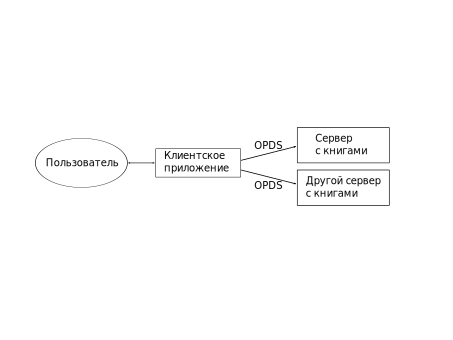
\includegraphics[width=.5\textwidth]{scheme}
%\caption{Мега-схема проекта}\label{fig:scheme}
%\end{figure}
%\picref{fig:scheme}	ссылка на картинку


\end{document}

